\section{Dynamic Programming}
From smaller subproblems to larger subproblems. 
\begin{enumerate}[-]
    \item \textbf{DAGs:} guarantees topological order, i.e. each  sub-problem only depends on previous sub-problem
    \item \textbf{Induction:} solve sub-problems in topological order, implemented by a for loop.
    \item \textbf{Memoization:} (not memorization)"backward" recursion with "storing"
\end{enumerate}
% \begin{figure}
%     \centering
%     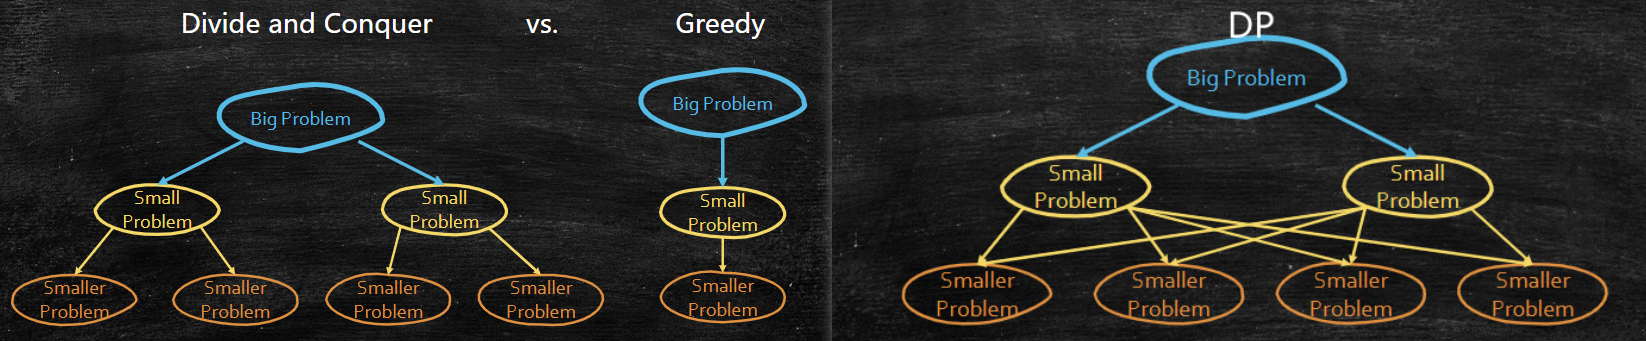
\includegraphics[width=0.5\linewidth]{DP.png}
% \end{figure}

Different from Divide and Conquer, where the scale decreases exponentially by a \textbf{'magic' merge operation}, 
DP reduces the scale a little bit.

Difference between Induction and Memoization: Theoretically, time-complexity is the same. 
Memoization has the advantage of not needing to compute \textbf{topological order}, and some \textbf{not-computed sub-problems}.
But in coding, 'throwing recursive call' is time costing.


\subsection{Longest Increasing Subsequence}
Formation of a DAG: establish a node i($i\in [1,n]$) for each element $a_i$, if $i<j$ and $a_i<a_j$, then $(a_1,a_j)\in E$.
Then the problem is to find the longest path in the DAG.
Construct L(i) by:
\[
    L(j)=1+\max{L(i):(i,j)\in E}\]
\textbf{Time Complexity} is $O(|V||E|)\leq O(n^2)$.\\
\textbf{Correctness of Algorithm} 

We'll prove that L(i) is the length of LIS ending at $a_i$.

For base step, L(0)=0 is the length of LIS for an empty sequence.

For induction step, assume that L(i) is the length of LIS ending at $a_i$, 
Let S be the LIS ending at $a_i$ and $T=S\backslash \{a_i\}$, the last number of $T$ is $a_t$.
Prove by $LIS[i]\geq |S|$, and $LIS[i]\leq |S|$.
Since $T$ is a LIS ending at $a_t$, $|T|=L(t)$, so $|S|=L(t)+1$. $L(i)=1+\max_{a_j<a_i,j<i}\{L(j)\}\geq L(t)+1=|S|$.

On the other hand, $L(i)=1+\max_{a_j<a_i,j<i}{L(j)+1}\leq 1+|T|=|S|$, so $L[i]\leq |S|$.

Therefore, $L(i)=|S|$.

\subsection{Edit Distance}
Edit distance is the minimum number of edits—insertions, deletions, and substitutions of characters—needed to transform
the first string into the second.
We denote $E(i,j)$ as the editing distance between $x[1..i]$ and $y[1..j]$.
\[
    E(i,j)=\min(1+E(i-1,j)+E(i,j-1)+E(i-1,j-1))
\]
diff(i,j)=0 iff x[i]=y[j].
Forming a $m \times n$ table, and each cell is computed only once, which results in \textbf{Time Complexity} of $O(mn)$.

\begin{algorithm}
    \caption{Edit Distance}
    \KwIn{Two strings $x[1..m]$ and $y[1..n]$}
    \KwOut{Edit distance $E(m,n)$}
    \For{$i=1$ to $m$}{
        $E(i,0)=i$\;
    }
    \For{$j=1$ to $n$}{
        $E(0,j)=j$\;
    }
    \For{$i=1$ to $m$}{
        \For{$j=1$ to $n$}{
            $E(i,j)=\min(1+E(i-1,j),1+E(i,j-1),diff(i,j)+E(i-1,j-1))$\;
        }
    }
    \Return{$E(m,n)$}\;
\end{algorithm}

Likewize, in the palindrome problem,
$H(i,j)$ to denote the biggest palindrome length.
\begin{equation}
H(i,j)= 
\begin{cases}
H(i+1,j-1)+2, & \text{if } A[i]=A[j],\\
\max\{H(i,j-1),H(i+1,j)\}, & \text{o.w.}
\end{cases}
\end{equation}

\subsection{Nnapsack Problem}
Denote $s[i]=v[i]/c[i]$, $s$ means the ratio of value to cost.
\begin{enumerate}
    \item indivisibility\\
    If it is divisible, if you choose the object with the largest xingjiabi each time, it is optimal, else you can switch two objects and get a better one, which results in a better solution 

    If it is indivisible, it is essentially an NP-Hard problem. As a problem where r of all objects are equal and v=totalSum/2 is a Partition Problem.
\end{enumerate}

For \textbf{time-complexity}, it is not a polynomial problem, with $O(nW)$, where W is a numerical value rather than size.

We can control the precision of $W$ by rounding, but the new optim solution you obtain may be infeasible in the original problem.

Howvever, if you round value, the feasibility of solutions doesn't change. 
Let $V=\max v_i$, $OPT\leq nV$. Denote $A[i,v]$ as the minimum cost cost(S) if we select till the $i^{th}$ item with exactly value $v$.
\begin{equation}
    A(i+1,v)= 
    \begin{cases}
    \min{A[i,v],c_{i+1}+A[i,v-v_{i+1}]} if v[i+1]<v\\
    A(i,v) & \text{o.w.}
    \end{cases}
\end{equation}

For \textbf{space-complexity}, it can be optimized from $O(nW)$ to $O(W)$.
A[1,v]=0 if v=0
c1 if v=v1
inf o.w.
\[
    f[i][v]=\max{f[i-1][v],f[i-1][v-c[i]]+w[i]}\]
Where $f[i][v]$ means putting the first $i$ objects into a $v$-capacity Knapsack. For every object $i$, you either put it in the bag, where the left capacity is $v-c[i]$, or not put it in, which is equal to $f[i-1][v]$.

\begin{remark}
    Fully Polynomial Time Approximation Scheme(FPTAS) gives a $(1-\epsilon)-$approximation with running time polynomial in term of $n$ and $\frac{1}{\epsilon}$

    Algorithms that can scale down the problem to constant length and use naive explore algorithm are commonly FPTAS.

    Polynomial Time Approximation Scheme(PTAS)
    gives a $(1-\epsilon)-$approximation with running time polynomial in term of $n$ and constant $\epsilon$.

    Some have fixed constant ratio
\end{remark}

